
\documentclass[
	%draft,
%	Entwurf,				% document will be marked as draft with current timestamp but all
							%graphics will be included
	%NoTableOfContents,		% do not create a Table Of Contents
	%NoListOfFigures,		% do not create a List Of Figures
	%NoListOfTables,			% do not create a List Of Tables
	USenglish 		 		% als Sprachen werden nur USenglish, ngerman und naustrian unterst�tzt!
	% ngerman
]{ACIN_diploma_thesis}

 \Title{\toolname: A graphical user interface for programming ROS based robots}
% \Subject{Diplomarbeit}
 \Author{Alexander Semeliker, BSc}
 \Date{29.07.2018}
 \PlaceAndTime{Wien, im September 2018}
 \AuthorAddress
 	{Georg Humbhandl Gasse 1\\
 	 2362 Biedermannsdorf\\
 	 \"Osterreich}
 \Supervisor{
 	Ao.Univ.-Prof.\@ Dipl.-Ing.\@ Dr.\,techn.\@ Markus\@ Vincze \\
 	% Dipl.-Ing.\@ Markus\@ Bajones
 }

%% PDFTitle nur notwendig, falls von Title abweichend. (Z.Bsp. falls Titel Zeilenumbr�che enth�lt)
% \PDFTitle{Title}
% \PDFAuthor{author}
% \PDFSubject{Diplomarbeit}


% Hinweise:
% - Beim drucken Seitenanpassung ausschalten!


% include necessary packages, add additional packages there!
\usepackage{booktabs}
\usepackage{tikz}

\usepackage{pgfplots}
\usetikzlibrary{pgfplots.groupplots}
\pgfplotsset{compat=1.9,height=0.3\textheight,legend cell align=left,tick scale binop=\times}
\pgfplotsset{grid style={loosely dotted,color=darkgray!30!gray,line width=0.6pt},tick style={black,thin}}
\pgfplotsset{every axis plot/.append style={line width=0.8pt}}

\usepgfplotslibrary{external}
% Für die Verwendung von 'external' müssen die folgenden Anpassungen in Abhängigkeit der
% LaTeX Distribution durchgeführt werden:

% fuer Texlive: pdflatex.exe -shell-escape -synctex=1 -interaction=nonstopmode %.tex
\tikzexternalize[shell escape=-shell-escape]   % fuer TeXLive

% fuer MikTeX:  pdflatex.exe -enable-write18 -synctex=1 -interaction=nonstopmode %.tex
%\tikzexternalize[shell escape=-enable-write18] % fuer MikTex



\tikzsetexternalprefix{graphics/pgfplots/} % Ordner muss ev. zuerst haendisch erstellt werden

\usepackage{enumerate}
\usepackage{color}

\definecolor{mygreen}{rgb}{0,0.6,0}
\definecolor{mygray}{rgb}{0.5,0.5,0.5}
\definecolor{mymauve}{rgb}{0.67,0.69,0.77}

\usepackage{listings}
\lstset{
    frame=tb,
    basicstyle=\fontsize{11}{13}\selectfont\ttfamily,
    captionpos=b,
    tabsize=2,
    numbers=left,
    xleftmargin=2em,
    framexleftmargin=1.5em,
    numberstyle=\color{mygray},
    stringstyle=\color{mygreen},
    morekeywords={with},
    keywordstyle=\bfseries\color{blue},
    abovecaptionskip=0.2em,
    breaklines=true,
    commentstyle=\color{mymauve},
    showstringspaces=false
}

\definecolor{darkgray}{rgb}{.4,.4,.4}
\definecolor{purple}{rgb}{0.65, 0.12, 0.82}
 
%define Javascript language
\lstdefinelanguage{JavaScript}{
    keywords={typeof, new, true, false, catch, function, return, null, catch, switch, var, if, in, while, do, else, case, break},
    keywordstyle=\color{blue}\bfseries,
    ndkeywords={class, export, boolean, throw, implements, import, this, init},
    ndkeywordstyle=\color{darkgray}\bfseries,
    identifierstyle=\color{black},
    sensitive=false,
    comment=[l]{//},
    morecomment=[s]{/*}{*/},
    commentstyle=\color{mymauve}\ttfamily,
    stringstyle=\color{mygreen}\ttfamily,
    morestring=[b]',
    morestring=[b]"
}

    
%define XML language
\definecolor{gray}{rgb}{0.4,0.4,0.4}
\definecolor{darkblue}{rgb}{0.0,0.0,0.6}
\definecolor{cyan}{rgb}{0.0,0.6,0.6}
\lstdefinelanguage{XML}
{
  morestring=[b]",
  morestring=[s]{>}{<},
  morecomment=[s]{<?}{?>},
  stringstyle=\color{black},
  identifierstyle=\color{darkblue},
  keywordstyle=\color{cyan},
  morekeywords={xmlns,version,type}% list your attributes here
}

% include file with settings
%\input{settings}

% sollte auskommentiert werden! (zum Anzeigen des Seitenspiegels auf der letzten Seite)
%\usepackage{layout}

% Alle externalisierten tikz/pgfplot Grafiken neu generieren:
%\tikzset{external/force remake}

\begin{document}

	% \input{macros.tex}
	\maketitle
	\lstlistoflistings
	
	% Include all the chapters...
	%=============================
%	\include{cha1_TemplateIntroduction}
%	\include{TestChapter}

	\chapter{Introduction}
	\chapter{Related Work}
This chapter examines the related work of fields this work is placed in. It starts with a brief summary of the fundamental development of \glspl{vpl}, then presents a classification of them and provides some representative examples. In the next section graphical environments for programming robots are summarized. Then an overview of researches and already existings \glspl{ui} is given. Finally, there is a comparison between matured interfaces with the one presented in this work.

\section{Visual Programming Languages}
There were basically two milestones in the development of an \gls{vpl} as we know it nowadays. The first milestone was Sketchpad, presented by Ivan Sutherland \cite{Sutherland:1963}. It was designed in 1963 on the TX-2 computer at MIT (Massachusetts Institute of Technology) and has been called the first computer graphics application. The system allowed users to work with a lightpen to create 2D graphics by creating simple primitives, like lines and circles, and then applying operations, such as copy, and constraints on the geometry of the shapes. Its graphical interface and support for user-specifiable constraints stand out as Sketchpad's most important contributions to visual programming languages. By defining appropriate constraints, users could develop structures such as complicated mechanical linkages and then move them about in real time.\cite{Boshernitsan:CSD-04-1368} David Canfield Smith achieved the next major, groundbreaking step in the history of \glspl{vpl}. In his PhD dissertation \cite{Smith:1975:PCP:907074} he introduced both the use of small pictorial objects, called icons, and the notion of programming by demonstration. \\

The field of \glspl{vpl} has grown rapidley in recent years and therefore more and more interest has been focused on creating a robust, standardized classification for work in the area. A lot of frameworks and environments are established in different fields of use, including education, multimedia, video games, simulation and automation processes. Since there are different focuses across these fields, the usage and design variies in a broad spectrum, and it is reasonable to classify them. As \cite{Boshernitsan:CSD-04-1368} outlines it is possible to cluster them according to the way users interact with them - e.g. differing \textit{purely visual languages} and \textit{hybrid text and visual systems}. Another appropiate classification scheme is the following, which focuses more on the data and input processing:

\begin{itemize}
    \item Block-based languages
    \item Flowcharts
    \item Dataflow programming languages
    % \item Finite-state machines
    % \item Behavior trees
\end{itemize}

\subsection{Block-based languages}
Block-based \glspl{vpl} are especially used in tools for reducing barriers for non-programmers or for teaching children programming. The core of these languages is a set of blocks, which can be connected with each other to form an executable program. Each block represents a specific paradigm of the proper programming language. A typical editor consists of a toolbox which contains the code blocks and a workspace, where the blocks can be placed - usually via a drag-and-drop, which is a key feature and make these \glspl{vpl} considered most intuitive and user-friendly.

The field of application of block-based \glspl{vpl} covers a wide range: Ardublock\footnote{http://blog.ardublock.com/} is a graphical programming add-on to the default Arduino \gls{ide} - an open-source electronics platform based on easy-to-use hardware and software, which has a broad community. The MIT App Inventor is a drag-and-drop visual programming tool for designing and building fully functional mobile apps for Android.\cite{AppInventor} In the fields of education Scratch\footnote{https://scratch.mit.edu/}, developed in 2007, plays an important role, since it is designed to be highly interactive. The name highlights the idea of tinkering, as it comes from the scratching technique used by hip-hop disc jockeys. In Scratch programming, the activity is similar, mixing graphics, animations, photos, music, and sound. The scripting area in the Scratch interface is intended to be used like a physical desktop (see \prettyref{fig:ScratchUI})\cite{Scratch}.

\begin{figure}[htbp]
	\centering
	\begin{overpic}[width=0.9\linewidth]{./graphics/ScratchUI}
	\end{overpic}
    \caption[Scratch user interface]%
            {Scratch user interface (Source:\cite{Scratch})}%
	\label{fig:ScratchUI}%
\end{figure}

\subsection{Flowcharts}
These \glspl{vpl} are able to translate an algorithm's logic given as flowchart into executable machine instructions. According to \cite{ISO2382} a flowchart is the graphical representation of a process or the step-by-step solution of a problem, using suitably annotated geometric figures connected by flowlines for the purpose of designing or documenting a process or program. Flowcharts are typically used in the fields of automation. Grafcet \cite{Grafcet} is a tool, drawing its inspiration from Petri nets (a general purpose mathematical tool allowing various discrete-event systems to be described), whose aim is the specification of \glspl{plc}. It is the basis of the \gls{sfc}, an International Standard in 1987. An implementation of the Grafcet norm can be found in S7-GRAPH, developed by Siemens AG and part of their STEP 7 software for programming \glspl{plc} (see \prettyref{fig:S7Graph}).

Another application using a flowchart \gls{vpl} is KTechLab\footnote{https://sourceforge.net/projects/ktechlab/}, which is an \gls{ide} for microcontrollers and electronics. It supports circuit simulation, program development for microcontrollers and simulating the programmed microcontroller together with its application circuit.

\subsection{Dataflow programming languages}
Similar to flowcharts dataflow programming is used for professional applications primarily, aimed at designers rather than end users or programmation beginners. Dataflow programming is a programming paradigm whose execution model can be represented by a directed graph, representing the flow of data between nodes, similarly to a dataflow diagram. Considering this comparison, each node is an executable block that has data inputs, performs transformations over it

\begin{figure}[!h]
% \begin{figure}[ht]
	\centering
	\begin{overpic}[width=0.65\linewidth]{./graphics/S7Graph}
	\end{overpic}
    \caption[S7-GRAPH interface of  STEP 7]%
        {S7-GRAPH interface of  STEP 7 (Source \footnotemark)}
        % {S7-GRAPH interface of  STEP 7 (Source \footnote{https://w3.siemens.com/mcms/simatic-controller-software/en/step7/simatic-s7-graph/pages/default.aspx})}
	\label{fig:S7Graph}%
\end{figure}
\footnotetext{https://w3.siemens.com/mcms/simatic-controller-software/en/step7/simatic-s7-graph/pages/default.aspx}

\begin{figure}[!h]
% \begin{figure}[!hb]
	\centering
	\begin{overpic}[width=0.65\linewidth]{./graphics/Simulink}
	\end{overpic}
    \caption[User interface of Simulink to use simulation models]%
    {User interface of Simulink to use simulation models (Source\footnotemark)}
    % {User interface of Simulink to use simulation models (Source\footnote{https://www.mathworks.com/products/simulink.html})}
	\label{fig:Simulink}%
\end{figure}
\footnotetext{https://www.mathworks.com/products/simulink.html}

and then forwards it to the next block. A dataflow application is then a composition of processing blocks, with one or more initial source blocks and one or more ending blocks, linked by a directed edge.\cite{Sousa2012DataflowPC} National Instruments LabVIEW \cite{LabView} and Simulink (\prettyref{fig:Simulink}) can be mentioned as the representatives of this big group.

\section{Graphical Robot Programming Environments} \label{sec:GraphicalEnvs}
The driving force of \glspl{vpl} in terms of graphical programming of robots is education. Teachers rely on simple educational robots and intuitive programming environments and graphical programming environments have become a frequent starting point for young students. The used environments mostly depends on the robot the corresponding class is programming and therefore there are many offerings. \\

A famous environment is the \textit{Lego Mindstorms} system\footnote{https://www.lego.com/en-us/mindstorms} - a hardware and software platform for the development of programmable robots based on Lego building bricks. It comes up with an \gls{ide} that is available on Windows PC or Mac. Its programming software is based on LabVIEW and provides the ability to downloading programs to the programmable brick, which can be connected to different sensors and actuators. Besides of the default editor the platform also supports the use of third-party environments as outlined in \cite{Hirst2003}. \\

Dataflow oriented \glspl{vpl}, like used in the mentioned Lego Mindstorms system, may be not suitable for absolute beginners, as described in \cite{Grape}. The author mention, that the procedural approach where a program is firstly considered as a sequence of statements is much easier to learn than the data flow or functional approach. Therefore a new graphical programming environment, called \textit{Grape}, was developed. With its help a flowchart can be built and the meaning of the individual elements of the flowchart are defined. It comes up with a list of predefined classes for robot programming and provides the feature to extend the list by own classes using a simple \gls{xml} syntax. The code generation itself also uses \gls{xml} representation: first the graphical structure of the program is converted into a \gls{xml} tree, which then is translated into \Cpp{} code via a mapping schema. \\

One of the most powerful graphical robot programming environment is the Open Roberta platform \cite{OpenRoberta}. The connection to the user is called \textit{Open Roberta Lab}, a cloud-­based application, which enables children and adolescents to visually program real robot hardware directly from the web browser or by using a build in online robot simulator. It also provides platform features like user login, program saving/sharing and easy hardware pairing over Wi-Fi as well as USB and Bluetooth connection.\cite{Ketterl_Jost_Leimbach_Budde_2015} Its programming language is called \textit{NEPO} and is built up on Google's Blockly, which also plays a fundamental part in this work (see \prettyref{sub:Blockly} and \prettyref{sec:CodeGeneration}). \\

When it comes to humanoid robots, by now, there are three major representatives: Nao\cite{Nao5152516}, Pepper\footnote{https://www.softbankrobotics.com/emea/en/pepper} and Romeo\footnote{https://projetromeo.com/}. All are developed by SoftBank Robotics and come up with a powerful \gls{sdk} called \textit{NaoQi}. Besides of \glspl{sdk} for Python, \Cpp{}, Java, JavaScript and \gls{ros}, the framework also provides a graphical programming tool: Choregraphe\cite{Choregraphe5326209}. Actually, Choregraphe is a specific module of NaoQi and more or less just a graphical representation of NaoQi's functions. The Choregraphe module produces an \gls{xml} file describing the program (i.e. the application, the boxes, the connections between them, the included scripts etc.). For execution, the file is interpreted by the XML module of NaoQi. Since the architecture of humanoid robots is very complex, even experienced programmers, at least partly, rely on interfaces like Choregraphe and therefore it is not exclusively used for education. \\

Another hybrid robot programming environment is provided by Aseba Studio\footnote{https://www.thymio.org/en:asebastudio} \gls{ide} of the Thymio II, a small and low-priced educational robot. It provides pure visual programming, two block based \gls{vpl} (Scratch, Blockly) as well as an editor and an \gls{api} for text programming. It is also possible to connect the robot an directly run and debug the program via the user interface.

\section{Environments for ROS-based robots} \label{sec:RosEnvs}
As stated in the beginning, \gls{ros} is considered as the de-facto standard framework for robot software development. Nonetheless the environments explained in \prettyref{sec:GraphicalEnvs}, as well as other frameworks too, does not provide \gls{ros} connectivity out-of-the-box.

This might be reasonable when thinking of purchasing a robot is not cheap. If an user needs to control just one robot, there is no necessity to search for a generic tool - especially because such a tool most likley would not provide as powerful capabilities as the default programming interface would do. Assuming the case of a lab, where several people might working with different robot or just quick showcases are desired, it is reasonable to design such an interface. Right now, there a only a few frameworks available for such purposes. \\

Erle Robotics developed a web-based visualization and block programming tool, called \textit{robot\_blockly}, which supports their own robots and drones \cite{erleblockly}. It comes preinstalled with their Linux-based artificial robotic brain \textit{Erle-Brain}\footnote{http://docs.erlerobotics.com/brains/erle-brain-3} and also provides a rudimentary interface for all other robots. It uses the standard block creation process of Blockly (\prettyref{sub:Blockly}). Therefore the user needs to update different files of the source code, must follow some naming rules, recompile Blockly and the package and also needs - apart from \gls{ros} - basic JavaScript knowledge. The \gls{ros} connectivity and all execution routines can be implemented in a Python file, which is read from a specific directory and then included into the Blockly source code. \\

Another Blockly-based tool for controlling \gls{ros}-based robots is the \textit{evablockly\_ros} package, developed by Inovasyon Muhendislik\cite{evablocklyros}. The provided blocks are mainly created specifically for operations that can be performed by using evarobot, a mobile robot platform built by the author. Apart from them the package also provides the following basic \gls{ros} connectivity features:

\begin{itemize}
	\item set up server connection
	\item create a publisher to send data
	\item send data via created publisher
	\item create a subscriber to receive data
	\item perform operations when data is received from determined subscriber
\end{itemize}

\section{Comparison of visual programming tools}
This section provides a comparison some visual programming tools presented in the previous sections with this work in respect of their features. The following systems were considered: robot\_blockly\cite{erleROS}, Choregraphe\cite{Choregraphe5326209}, Open Roberta Lab\cite{Ketterl_Jost_Leimbach_Budde_2015}, Grape\cite{Grape} and EV3\cite{LegoEV3}. The specified features aiming two important fields of the tool decision process - platform independency and usablity. Those two main features are broken down to several minor criterias, as \prettyref{tab:Comparison} shows. All of the mentioned tools come with an \gls{ide} for multiple computer platforms and operation systems. \\

Most of the tools provide a block-based programming interface, which tends to be the simplest \gls{vpl} type in terms of usablity. Conclusively, the two most popular educational programming platforms, EV3 - the newest generation of the Lego Mindstorms system - Open Roberta Lab, are included. Since EV3 also provides the ability to use third-party environments, all \glspl{vpl} are supported as well as pure coding itself. When looking at the provided programming options of Choregraphe, it is highlighted that it is possible to create complex programms with it, but getting there requires more technical expertise. The tool presented in this work, \toolname{}, trys to reach both audiences. \\

Open Roberta Lab supports seven different robot platforms out of the box, which is significantly more than the other tools. Besides its own programming brick, EV3 supports its
preceding robot system NXT partially at the moment, but allows the integration of third-party sensors and motors. Choregraphe Suite supports platforms providing the NaoQi \gls{sdk}, which are currently three physical robots. All other tools only provide connectivity to one robot though, but are able to be upgraded via different interfaces. Only \toolname{} comes up with an assistent, the others require to touch or recompile the source code. \\

Besides the number of robots, which can be connected to a system, platform independency also means, that different operating systems are supported. Web-based applications are the most independent ones, since users are not required to install software on their computers. Running the infrastructure on a server allows users to connect to the robot remotely and use it on mobile devices too. EV3 currently supports mobile devices with the following minimum versions: Android 4.2, iOS 8.0. Of the evaluated tools \toolname{}, robot\_blockly and Open Roberta Lab are fully web-based. All of them are based on Google's Blockly framework. \\

Development support interfaces such as a robot simulatior and a debugging tool are only provided by two tools. When comparing this to the programming types, a pattern could be obatined. One of the advantages using a block-based \gls{vpl} is that the translated code is always syntactically correct, so a major reason using such support during development, is obsolete. \\

When it comes to \gls{ros} connectivity the classification outlined in \prettyref{sec:GraphicalEnvs} and \prettyref{sec:RosEnvs} can be applied. Except EV3 it is possible to create \gls{ros} nodes with each tool. It is worthy of remark thaht Choregraphe's NaoQi \gls{sdk} provides \gls{ros} connectivity only via code represention, i.e. it is not possible to use \gls{ros} communication within the graphical programming interface. Of the tools enabling updates for both \gls{ros} connectivity and robot platforms, all provide a manual, but only the workflow of \toolname{} is tool assisted. This means that upgrading is more of a configuration than programming process - depending on how complex the desired block should be. Therefore less programming knowledge is required - especially in terms of the communication patterns of \gls{ros}. Not touching the source code also means no recompiling, which therefore leads to the fact, that - once deployed - \toolname{} runs autonomously without any internet connection required.

\def\rotdeg{90}
\begin{table}[htbp]
	\begin{minipage}{\textwidth}
		\centering
		\begin{tabular}{l | l | c c c c c c}
			\multicolumn{2}{c}{Feature} & \rotatebox{\rotdeg}{\toolname{}} & \rotatebox{\rotdeg}{robot\_blockly} & \rotatebox{\rotdeg}{Choregraphe} & \rotatebox{\rotdeg}{Open Roberta Lab} & \rotatebox{\rotdeg}{Grape} & \rotatebox{\rotdeg}{EV3} \\
			\toprule
			\multirow{4}{*}{Programming} & block-based & \checkmark & \checkmark & & \checkmark & & \checkmark \\
			& flowchart & & & & & \checkmark & \checkmark \\
			& dataflow & & & \checkmark & & & \checkmark \\
			& code & \checkmark & & \checkmark & & & \checkmark \\
			\hline
			\multirow{2}{*}{Robot platforms} & out-of-the-box & 1 & 1 & 1 & 7 & 1 & 2\footnote{third-party sensors and motors are supported} \\
			& upgradeable & \checkmark & \checkmark &  & \checkmark & \checkmark & \\
			\hline
			\multirow{4}{*}{User interface} & upgrade assistent & \checkmark & & & & & \\
			& web-based & \checkmark & \checkmark &  & \checkmark & & \\
			& simulator & & & \checkmark & & & \\
			& debugging & & & \checkmark & & & \checkmark \\
			\hline
			\multirow{2}{*}{\gls{ros} connectivity} & out-of-the-box & \checkmark & \checkmark &  &  & & \\
			& upgradeable & & & (\checkmark)\footnote{not for visual programming environment} & \checkmark & \checkmark &\\
			\hline
			\multirow{4}{*}{Upgrade workflow} & tool assisted & \checkmark & & - & & & -\\
			& manual & \checkmark & \checkmark & - & \checkmark & \checkmark & -\\
			& programming languages & 1 & 2 & - & 2 & 2 & - \\
			& recompiling & & \checkmark & - & \checkmark & & - \\
			\bottomrule
		\end{tabular}
		\caption{Comparison of visual programming platforms}
		\label{tab:Comparison}
	\end{minipage}
\end{table}

% \section{Choregraphe}

% \section{evablockly\_ros - Inovasyon Muhendislik}

% \section{robot\_blockly - erlerobotics}

% \section{RobotC}
	\chapter{Architecture}
This chapter describes the architecture and implementation of \toolname{} (portmanteau of ROS and Blockly). First the purpose and need of it are explained, followed by a architectural overview of \hobbit{}, the used robot. Based on this constraints the options implemtenting the tool are presented as well as an explanation of the decision. Then a short description of the robot operating system ROS and the fundamental JavaScript frameworks, Node.js and Express, are given and finally the necessary details of the implementation are documented - for both, the frontend and the backend.

\section{Requirements} \label{sec:requirements}
In the field of software engineering constraints are the basic design parameters. Therefore it is necessary to provide them as detailed as possible. In the given case the basic constraints are given by the purpose of the tool and the architecture of the robot.

\subsection{\hobbit{} - The Mutal Care Robot}
The HOBBIT PT2 (prototype 2) platform was developed within the EU project of the same name. The robot was developed to enable independent living for older adults in their own homes instead of a care facility. The main focus is on fall prevention and detection. PT2 is based on a mobile platform provided by Metralabs. It has an arm to enable picking up objects and learning objects. The head, developed by Blue Danube Robotics, combines the sensor set-up for detecting objects, gestures, and obstacles during navigation. Moreover, the head serves as emotional display and attention center for the user. Human-robot interaction with Hobbit can be done via three input modalities: Speech, gesture, and a touchscreen. \cite{HobbitACIN}\\

\begin{figure}[htbp]
	\centering
	\begin{overpic}[width=0.3\linewidth]{./graphics/Hobbit}
	\end{overpic}
	\caption{\hobbit{} - The Mutal Care Robot}%
	\label{fig:HobbitPic}%
\end{figure}

In terms of technology \hobbit{} (see \prettyref{fig:HobbitPic}) is based on the robot operating system ROS (\prettyref{sub:ros}), which allows easy communication between all components. The system is set up to be used on Ubuntu 16.04 together with the ROS distribution \textit{Kinetic}. All ROS nodes are implemented in either Python or \Cpp{}. In order to provide a fast and simple way to implement new behaviours several commands should be pre-implemented. These commands are performed either by publishing messages to topics or services, or executing callbacks defined in the corresponding action's client. The common commands and their description are listed in \prettyref{tab:hobbitCommands}. A detailed list of possible messages for each command will be presented in \prettyref{sub:ros} after furher explanation of the ROS architecture.

\begin{table}
	\centering
	\begin{tabular}{l l l l}
		\toprule
		Name               & Type    & Message type               & Description            \\
		\midrule
		/cmd\_vel          & Topic   & geometry\_msgs/Twist       & move \hobbit           \\
		/head/move         & Topic   & std\_msgs/String           & move \hobbit's head    \\
		/head/emo          & Topic   & std\_msgs/String           & control \hobbit's eyes \\
		/MMUI              & Service & hobbit\_msgs/Request       & control UI interface   \\
		hobbit\_arm        & Action  & hobbit\_msgs/ArmServer     & control \hobbit's arm  \\
		move\_base\_simple & Action  & geometry\_msgs/PoseStamped & navigate \hobbit       \\
		\bottomrule
	\end{tabular}
	\caption{Common commands used by \hobbit}
	\label{tab:hobbitCommands}
\end{table}

\subsection{Purpose of the tool}
\hobbit{} became very popular since the above mentioned EU project and demos of it's behaviours has been presenting at large number of fairs. Unfortunally only the following show cases are currently implemented on the robot:

\begin{itemize}
	\item \hobbit{} follows the user
	\item \hobbit{} learns object
	\item \hobbit{} starts an emergency call
	\item \hobbit{} picks up an object
\end{itemize}

All of the demos can be started via the UI running on \hobbit{}'s tablet, but re-writing new demos would assume a detailed knowledge of the robot's setup. In order to implement new behaviours and demos more easily it is necessary to provide a programming interface, which provides a powerful, generic base to cover a wide range of \hobbit's features as well as an intuitive handling.\\

Furthermore the \ACIN{} of the TU Wien is part of the Educational Robotics for STEM (ER4STEM) project, which aims to turn curious young children into young adults passionate about science and technology with hands-on workshops on robotics. The ER4STEM framework will coherently offer students aged 7 to 18 as well as their educators different perspectives and approaches to find their interests and strengths in robotics to pursue STEM careers through robotics and semi-autonomous smart devices. \cite{ER4STEMACIN} Providing an intuitive programming tool would allow the integration of \hobbit{} into the project, which would be an extra input evaluation parameter.\\

At last the framework should be implement to be re-used for other ROS based robots. This means, that it should not only provide an interface to the mentioned commands for \hobbit{}, but an open, adpatable framework. It should be able to allow a flexible configuration and assembly of the provided functions.

\section{Options}
There are several approaches to fulfill the mentioned requirements. In the following subsections three different options are presented by a simple example: the implementation of picking up an object from the floor an putting it on the table. This should give a rough overview in terms of complexity of the usability as well as the implementation of the corresponding approach. For reasons of simplicity tasks like searching and detecting the object or gripper positioning are excluded.

\subsection{Custom API}
\label{sub:PyApi}
The most obvious way to fulfill the requirements is to provide an application programming interface (API) for the desired programming languages (Python, \Cpp{}). An API is a set of commands, functions, protocols, and objects that programmers can use to create software or interact with an external system. It provides developers with standard commands for performing common operations so they do not have to write the code from scratch. In the present case such a API could consists of the following components:

\begin{itemize}
	\item Initialization: setting up communication and intial states - e.g. creating ROS nodes, starting the arm referencing or undocking from charger
	\item Topic management: managing the messages published to ROS topics and creating subscriber nodes if applicable
	\item Service management: managing the ROS services of \hobbit{} - e.g. the tablet user interface
	\item Action management: creating ROS action clients for e.g. navigation or arm movement
	\item Common commands: providing common commands (see \prettyref{tab:hobbitCommands})
\end{itemize}

It should be noted, that the components doesn't re-implement ROS functionality, but extend it and prvovide a simpler use of it. Depending of how generic the API is implemented it is possible that the user can control the robot without any detailed knowledge of the technical setup of it. Nevertheless this approach would assume the user to have knowledge of the programming language the API is desigend for. Refering to the required commands in \prettyref{tab:hobbitCommands} an API for Python could be designed as shown in \prettyref{fig:PythonApi}. The highest usability would be reached, if all input parameters are from common variable types such as interger and string. Indeed, this would increase the implementation effort, especially in terms of error handling, as well as the extent of the documentation,  which are huge disadvantages of writing an API. \\

\begin{figure}[htbp]
	\centering
	\begin{overpic}[width=0.8\linewidth]{./graphics/PythonApi}
	\end{overpic}
	\caption{Exemplary design of API for Python}%
	\label{fig:PythonApi}%
\end{figure}

Assuming the API would be implemented as explained before and the Python module would be named \textit{HobbitRosModule}, \prettyref{lst:PythonApiEx} shows a sample code for the mentioned use case to pick up an object. Note that the code is very short and easy to read, which - on the other hand - means that the implementation of the API must cover a broad technical range, such as error handling for unsupported inputs and communication errors.

\begin{figure}[htbp]
	\lstinputlisting[label={lst:PythonApiEx},caption={Example Python code using the API shown in \prettyref{fig:PythonApi}}, language={Python}]{./listings/PythonApiEx.py}
\end{figure}

\subsection{\smach{}}
\smach{} is a task-level architecture for rapidly creating complex robot behavior. At its core, \smach{} is a ROS-independent Python library to build hierarchical state machines. \cite{SmachROS}. Since that, this approach would also end up in providing an API for the user, but allows to create more complex demos with less effort than the one described in \prettyref{sub:PyApi}. \smach{} also provides a powerful graphical viewer to visualize and introspect state machines as well as an integration with ROS, of course. Since the aforementioned example is a very simple one and doesn't require a lot of the provided \smach{} functionality, this section only covers the needed ones to fulfill the requirements. For a detail description on how to use \smach{} refer to \cite{SmachROS}. \\

The arm of \hobbit{} is controlled via the hobbit\_arm action. \smach{} supports calling ROS action interfaces with it's so called \textit{SimpleActionState}, a state class that acts as a proxy to an \textit{actionlib} (see \prettyref{sub:ros}) action. The instantiation of the state takes a topic name, action type, and some policy for generating a goal. When a state finishes, it returns a so called \textit{outcome} - a string that describes how the state finishes. The transition to the next state will be specified based on the outcome of the previous state. \prettyref{lst:SmachExCode} shows a possible implementation of picking up a object an placing it on the table. After the imports of the necessary modules (lines 1 to 4), the state machine is instanced (line 7), to which the required states are added (lines 17-22). The parameters passed to \textit{SimpleActionState} are

\begin{itemize}
	\item the name of the action as it will be broadcast over ROS (e.g. \textit{hobbit\_arm})
	\item the type of action to which the client will connect (e.g. \textit{ArmServerAction}) and
	\item the goal message.
\end{itemize}

For reasons of readability the goals are declared at a seperate code block (lines 11 to 14). The equivalent visualization of the state machine is shown in \prettyref{fig:SmachSM}. \\

\begin{figure}[htbp]
	\lstinputlisting[label={lst:SmachExCode},caption={Using \smach{} to generate a state machine}, language={Python}]{./listings/SmachEx.py}
\end{figure}

\begin{figure}[htbp]
	\centering
	\begin{overpic}[width=0.7\linewidth]{./graphics/SmachSM}
	\end{overpic}
	\caption{State machine generated via \prettyref{lst:SmachExCode}}%
	\label{fig:SmachSM}%
\end{figure}

Providing just the \smach{} interface has some disadvantages and would not be practicable. First the user would need an advanced knowledge of Python. Depending on the design of the self-implemented API (\prettyref{sub:PyApi}) the knowledge has to be at least at the same level. Next the user would have to understand the API and needs to find a design to fit for the corresponding demo case. Furthermore it requires the user also to exactly know the ROS specification of the robot. So, if \smach{} would be choosen as the underlying framework, it would also be necessary to provide a more abstract API - basically with the same interfaces as shown in \prettyref{fig:PythonApi}.

\subsection{Blockly}
Blockly is a library that adds a visual code editor to web and Android apps. The Blockly editor uses interlocking, graphical blocks to represent code concepts like variables logical expressions, loops, and more. It allows users to apply programming principles without having to worry about syntax or the intimidation of a blinking cursor on the command line. \cite{BlocklyIntro} So for the present case, in contrast to the other approaches the user would not need to have any technical knowledge of \hobbit{}, it's components and interfaces. Furthermore such a editor would not require the user to master any programming language. On the other hand implementing this approach would require knowledge of web applications (i.e. JavaScript, HTML and CSS) additionally. \\

\begin{figure}[htbp]
	\centering
	\begin{overpic}[width=0.9\linewidth]{./graphics/BlocklyEx}
	\end{overpic}
	\caption{A short Blockly demo showing it's structure and use}%
	\label{fig:BlocklyEx}%
\end{figure}

\prettyref{fig:BlocklyEx} shows an exemplary injection and use as well as the basic structure of Blockly applications. It consists of a toolbox, from where the progamming blocks can dragged to the workspace, where they are connected. The Blockly API \cite{BlocklyAPI} provides a function to generate code for all blocks in the workspace to several languages: JavaScript, Python, PHP, Lua, Dart and XML. In the shown example for each of them a tab is avaible to show the generated code. The blocks dragged to the workspace in \prettyref{fig:BlocklyEx} are already customized blocks, with whom an object can be picked up and be placed on the table. There are basically four steps requierd in order to create and use a custom block, which are described briefly in the following paragraphs. A detailed documentation is given in \cite{BlocklyCustomBlocks}.

\subsubsection{Defining the block}
Blocks are defined in the \textit{blocks} directory of the source code by adding either JSON objects or JavaScript functions to the \lstinline!Blockly.Blocks! mapping. It includes the specification of the shape, fields, tooltip and connection points. An exampe definition using a JavaScript function of the \textit{gripper} block is shown in \prettyref{lst:DefineBlockEx}. Attention should be payed to lines 6 to 21, where the input fields are defined (line 8). Here a dropdown field with two options ("Open" and "Close") is created. The name ("gripper\_position") is used to refer to it later.

\begin{figure}[htbp]
	\lstinputlisting[label={lst:DefineBlockEx},caption={Block initialization using a JavaScript function}, language={JavaScript}]{./listings/BlocklyBlockInitEx.js}
\end{figure}

\subsubsection{Providing the code}
Similar to the definition of a block, the code, which is generated out of them, is stored in a mapping variable inside the Blockly library. Since different languages are supported, the code definition has to be in the right directory. Note that it is not necessary to provided code for each language. The code generation is handled in the \textit{generator} directory of the library. Each language has it's own helper functions file (e.g. \lstinline!python.js!) and subdirectory, where the code for each block is defined. There are several interfaces functions provided by Blockly to manage interaction with a block - such as collecting arguments of the block. A short example to control \hobbit{}'s gripper is shown \prettyref{lst:DefineCodeEx}. In line 2 the \lstinline!block.getFieldValue()! function is used to get the user's selection of the dropdown field. Note that the generator always returns a string variable including the code in the desired language (line 4). So the shown example requires to use a custom Python API (such as \prettyref{fig:PythonApi}), because \lstinline!node.gripper()! is not a built-in function of Python. \\

\begin{figure}[htbp]
	\lstinputlisting[label={lst:DefineCodeEx},caption={Defintion of a code generator in Blockly for Python}, language={JavaScript}]{./listings/BlocklyCodeInitEx.js}
\end{figure}

\subsubsection{Building}
After the customized block and it's code generator are defined, the whole Blockly project has to be rebuilt by running \lstinline!python build.py!. Building means that the source code, which is usually spread to several - in the given case over a hundred - files, is converted into a stand-alone form, that can be easily integrated. The Blockly build process uses Google's online Closure Compile and outputs compressed JavaScript files for core functionalites, blocks, block generators for each progamming language and a folder including JavaScript files for messages in several lingual languages. In our case the following four files needs to be included:

\begin{itemize}
	\item \lstinline!blockly_compressed.js!: Blockly core functionalites
	\item \lstinline!blocks_compressed.js!: Defintion of all blocks
	\item \lstinline!python_compressed.js!: Code generators for all blocks
	\item \lstinline!/msg/js/en.js!: English messages for e.g. tooltips
\end{itemize}

\subsubsection{Add it to the toolbox}
Once the building is completed and the necessary files are included to the web application, the custom block needs to be included in the toolbox. The toolbox is specified in XML and passed to Blockly when it is injected. Assuming the blocks shown in \prettyref{fig:BlocklyEx} are build as described in the previous paragraphs, they can be add to the toolbox as shwon in \prettyref{lst:DefineToolboxEx}. \\

\begin{figure}[htbp]
	\lstinputlisting[label={lst:DefineToolboxEx},caption={Minimal example of adding two blocks to a Blockly toolbox}, language={XML}]{./listings/BlocklyToolboxEx.xml}
\end{figure}

\subsection{Decision}
In order to select the best fitting solution the requirements explained in \prettyref{sec:requirements} are summarized as follows:

\begin{itemize}
	\item The user wants to build as complex demos as possible.
	\item The user wants an intuitive interface to create demos.
	\item The user should need as little knowledge of the robot as possible.
	\item The user should need as little technical knowledge as possible.
	\item The implementation of the tool should not exceed the usual effort of a master thesis.
	\item The tool should provide the ability to add new functionalites.
	\item The tool should be maintable, meaning it should have clear interfaces and as less dependencies as possible.
\end{itemize}

The selection is based on rating each of the approaches in regards of each single requirement mentioned with a score ranging from 0 (lowest) to 5 (highest). The approach with the highest overall score is seen as the best fitting one and will be implemented. \prettyref{tab:decision} shows the result of the evaluation. In the end the Blockly convinced with its very intuitive interface, which requires the user to have very little previous knowledge to build demos. Despite the fact that maintainability and scalability suffer from the high abstraction and encapsulation of the libary, the effort in terms of implementation is not worth mentioning compared to the other approaches. This results from the circumstance each one would require the design of a custom API. Instead of just abstracting the given ROS functionality, Blockly adds a much more user-friendly option to create demos - in contrast to the others.

\begin{table}[htbp]
	\centering
	\begin{tabular}{l c c c}
		\toprule
		                        & Custom API & \smach{} & Blockly \\
		\midrule
		Complexity of demos     & 3          & 4        & 2       \\
		User Interface          & 2          & 2        & 5       \\
		Robot specific know-how & 3          & 1        & 5       \\
		Technical know-how      & 1          & 1        & 5       \\
		Implementation          & 2          & 3        & 3       \\
		Scalability             & 4          & 3        & 2       \\
		Maintainability         & 3          & 3        & 1       \\
		% Dependencies            & 4                 & 2        & 2       \\
		\bottomrule
		$\Sigma$                & 18         & 17       & 23      \\
		\bottomrule
	\end{tabular}
	\caption{Evaluation of possible approaches}
	\label{tab:decision}
\end{table}

\section{Frameworks}
The fundamental component of \toolname{}'s architecture (\prettyref{fig:Architecture}) is a custom Python module, which abstracts ROS commands, but there are also several other basic frameworks used and it's necessary to have a brief overview of them.

\begin{figure}[htbp]
	\centering
	\begin{overpic}[width=\linewidth]{./graphics/Architecture}
	\end{overpic}
	\caption{Frontend and backend architecture of \toolname{}}%
	\label{fig:Architecture}%
\end{figure}

\subsection{ROS} \label{sub:ros}
ROS (Robot Operating System) provides libraries and tools to help software developers create robot applications. It provides hardware abstraction, device drivers, libraries, visualizers, message-passing, package management, and more. Since ROS is licensed under an open source, BSD license it used for a wide range of robots, sensors and motors. Covering all of its features would go beyond the scope of this thesis, so just the concepts, which are needed to implement \toolname{}, are summarized. \cite{WikiROS}

\subsubsection{Packages}
Software in ROS is organized in packages. A package might contain ROS nodes, a ROS-independent library, a dataset, configuration files, a third-party piece of software, or anything else that logically constitutes a useful module. The goal of these packages it to provide this useful functionality in an easy-to-consume manner so that software can be easily reused.

\subsubsection{Nodes}
A node is a process that performs computation and are written with the use of a ROS client library, such as roscpp (for \Cpp{}) or rospy (for Python). Nodes are combined together into a graph and communicate with one another using streaming topics, RPC (Remote Procedure Call) services, and the Parameter Server. A robot control system will usually comprise many nodes. For example, one node controls a laser range-finder, one Node controls the robot's wheel motors, one node performs localization, one node performs path planning, and so on.

\subsubsection{Topics}
Topics are named buses over which nodes exchange messages. Topics have anonymous publish/subscribe semantics, which decouples the production of information from its consumption. In general, nodes are not aware of who they are communicating with. Instead, nodes that are interested in data subscribe to the relevant topic; nodes that generate data publish to the relevant topic. There can be multiple publishers and subscribers to a topic. Each topic is strongly typed by the ROS message type used to publish to it and nodes can only receive messages with a matching type.

\subsubsection{Messages}
A message is a simple data structure, comprising typed fields. Standard primitive types (integer, floating point, boolean, etc.) are supported, as are arrays of primitive types. Messages can include arbitrarily nested structures and arrays. Nodes can also exchange a request and response message as part of a ROS service call. Message descriptions are stored in .msg files in the msg/ subdirectory of a ROS package.

\subsubsection{Services}
The publish-subscribe model is a very flexible communication paradigm, but its many-to-many one-way transport is not appropriate for RPC request-reply interactions, which are often required in a distributed system. Request-reply in ROS is done via a service, which is defined by a pair of messages: one for the request and one for the reply. Services are defined using .srv files, which are compiled into source code by a ROS client library.

\subsubsection{Actions}
In some cases, e.g. if a service takes a long time to execute, the user might want the ability to cancel the request during execution or get periodic feedback about how the request is progressing. The actionlib package provides tools to create servers that execute long-running goals that can be preempted. It also provides a client interface in order to send requests to the server.
The action client and action server communicate via a "ROS Action Protocol", which is built on top of ROS messages. The client and server then provide a simple API for users to request goals (on the client side) or to execute goals (on the server side) via function calls and callbacks.

\subsection{Node.js \& Express}

\subsection{Others}

\section{Frontend implementation}
\subsection{Demo Management}
\subsection{Code Generation}
\subsection{Code Editor}
\subsection{Backend Communication}
\section{Backend implementation}
\subsection{Frontend Communication}
\subsection{Storage Management}
\subsection{Python module}
\subsection{Code Execution}
	\chapter{Implementation}
This chapter gives detail insights into the implementation of \toolname{}. Each component presented in the architectural overview (\prettyref{sec:ArchitectureOverview}) is explained together with the essential code snippets.

\section{Backend \& Frontend Communication}
The communication between frontend (client) and backend (server) is done via a RESTful \gls{api}. A RESTful \gls{api} is based on representational state transfer (REST) technology and uses HTTP (Hypertext Transfer Protocol) request methods, which are defined in RFC 2616 \cite{RFC2616}, to exchange data between web services. All implemented \gls{api} endpoints, which are used to manage demos and codes are listed in \prettyref{tab:APIspec}.

\begin{table}[htbp]
	\centering
	\begin{tabular}{l l l}
		\toprule
		Type   & Path                               & Description                                     \\
		\midrule
		GET    & /demo/list                         & list all demos saved on the robot               \\
		GET    & /demo/load/\textit{\{demoId\}}     & get the \gls{xml} tree of a demo        \\
		POST   & /demo/save                         & save a new demo on the robot                    \\
		POST   & /demo/run/\textit{\{demoId\}}      & run a demo                                      \\
		DELETE & /demo/delete\textit{\{demoId\}}    & delete a demo                                   \\
		GET    & /demo/toolbox                      & load the toolbox of the Blockly interface       \\
		GET    & /block/list                        & list all already configured custom blocks       \\
		POST   & /block/create                      & create a new custom block                       \\
		PUT    & /block/update/\textit{\{blockId\}} & update a custom block                           \\
		DELETE & /block/delete/\textit{\{blockId\}} & delete a custom block                           \\
		\bottomrule
	\end{tabular}
	\caption{API endpoints for managing demos and custom blocks}
	\label{tab:APIspec}
\end{table}

\section{Demo Management}
The Demo Management (\prettyref{fig:DemoManagement}) is one key feature of \toolname{} and the entry point of it. It gives an overview of all avaible demos, meaning demos, which are saved on the robot in a specific directory. It provides a graphical interface and hence makes it a lot easier to manage and run demos - in contrast to the other mentioned options (\prettyref{sec:Options}), where e.g. the user needs to explicity locate the file and run it. Since usability and simplicity are main requirements for this tool, such a feature is a main advantage of it. Furthermore the main page provides the option to create new demos and a redirection to the block configuration component (\prettyref{sec:BlockConfiguration}).

\begin{figure}[htbp]
	\centering
	\begin{overpic}[width=\linewidth]{./graphics/DemoManagementFrontend}
	\end{overpic}
	\caption{Demo Management Page}%
	\label{fig:DemoManagement}%
\end{figure}

At the start of the tool the \lstinline!/demos/! directory inside the tools folder on the robot is searched for saved demos. Since we talking about a web-based tool and demos are saved on the robot, this requieres a call to the backend, which then returns a list of all demos via the RESTful \gls{api}. The structure of all demos are stored in \lstinline!.xml! files, which are interpreted by Blockly.

\section{Block Configuration} \label{sec:BlockConfiguration}
There are a lot of needs a user want to create a custom block. The pre-implemented blocks are designed for the \gls{ros} architecture of \hobbit{} and any other robot won't show the desired behavior when receiving commands sent from these blocks. Even for \hobbit{} itself the provided block set doesn't cover all of its functionalites. Using another robot means publishing different data to other topics, calling other services and using other action clients. Of course, the user can walk through the whole custom block creation process described in \prettyref{sub:Blockly} to create new blocks. This requieres knowledge of progamming in JavaScript and the Blockly \gls{api}. The user would then can use all of Blockly's broad range of features and advantages, especially dynamically changing of block features.

On the other hand for a lot of the tasks such features aren't necessary or a workaround with less effort can be found, respectively. For this reason \toolname{} provides a block configuration interface, which allows the user to create custom blocks with the two basic visual designs: an execution block and an input block (\prettyref{fig:CustomBlockTypes}). With this interface the user can configure blocks for publishing data to topics, calling services with parameters and creating simple action clients.

\begin{figure}[htbp]
	\centering
	\begin{overpic}[width=0.5\linewidth]{./graphics/ExCustomBlockTypes}
	\end{overpic}
	\caption{Basic visual designs: execution block (left) and input block (right)}%
	\label{fig:CustomBlockTypes}%
\end{figure}

The design of the interface is shown in \prettyref{fig:BlockConfiguration}. It is devided into three sections:
\begin{enumerate}[I.]
	\item An overview of already created custom blocks
	\item A form to provide general information of the block
	\item A form to provide detail information of the block (type-specific)
\end{enumerate}

\begin{figure}[htbp]
	\centering
	\begin{overpic}[width=0.8\linewidth]{./graphics/BlockConfiguration}
	\end{overpic}
	\caption{Design of the block configuration interface}%
	\label{fig:BlockConfiguration}%
\end{figure}

The list of all already configured custom blocks is loaded via the GET request endpoint \lstinline!/block/list! of the tool's internal RESTful \gls{api}. The request delivers an object with the Blockly conform block and code definitions, the unique ID and name of the respective block as well as the block's meta data. The latter is used to set the general and detail forms in case the custom block is selected. Identification which custom block is selected is handeld via the query string of the URL, which is set to the custom block's ID if it is selected. The ID of a block is a alphanumerical 12-character string, which is generated randomly. \\

The general information form is primarily used to set the visual design of the block. The user can configure the title and tooltip of the block as well as the number and names of the inputs, which then can be used in the detail section. The detail section varies depending on which type of the \gls{ros} communicating patterns is used. A topic must be specified by its name, the message type and the message itself. If the user wants to create a custom block for calling services, it is necessary to provide the name of the service, the message type and a list of all message type specific fields with their values. Furthermore it is possible to choose whether the response of the service should be used as output - which will lead to an input block - or not - then an execution block is generated (\prettyref{fig:CustomBlockTypes}). The detail section for actions includes fields for setting the execution timeout (which is defined as the time to wait for the goal to complete), the server name, the message type and the goal. It is also possible to provide the following callback functions:

\begin{itemize}
	\item done\_cb: callback that gets called on transitions to  \textit{Done} state.
	\item active\_cb: callback that gets called on transitions to  \textit{Active} state.
	\item feedback\_cb: callback that gets called whenever feedback for the goal is received.
\end{itemize}

All detail sections also features an input field for importing all Python packages that are needed to execute the code correctly, e.g. messages types that are used to generate the message. Some step-by-step examples for configuring custom blocks are presented in \prettyref{apx:BlockConfigManual}.

\section{Code Generation} \label{sec:CodeGeneration}
Demos are created via the user interface shown in \prettyref{fig:CodeGeneration}. It can be devided into three sections:

\begin{enumerate}[I.]
	\item the \textbf{navigation header} holds elements to directly manage the current demo,
	\item the \textbf{toolbox} contains code blocks organized in categories,
	\item the \textbf{workspace} where the blocks can be dragged to from the toolbox and connected with each other.
\end{enumerate}

\begin{figure}[htbp]
	\centering
	\begin{overpic}[width=\linewidth]{./graphics/CodeGenerationScreen}
	\end{overpic}
	\caption{User interface for demo and code generation}%
	\label{fig:CodeGeneration}%
\end{figure}

Blocks which are dragged to and combined at the workspace creates are used to generate an executable code. This is done with the help of Blockly (see \prettyref{sub:Blockly}). Blockly came up with some predefined code blocks that allow some basic programming procedures.
On top of them \toolname{} provides further blocks, which allows to connect to \hobbit{} and perform several actions (\prettyref{tab:hobbitCommands}). A list and description of these blocks can be found in \prettyref{apx:BlockOverview}. All of them are using one of the mentioned \gls{ros} communicating pattern (topic, service, action) to call the interface of the robot and have a similar structure thanks to the design of a custom Python module (\prettyref{sec:PythonModule}). \\

To get a clearer understanding of the general structure of these blocks and the Blockly custom block creation (\prettyref{sub:Blockly}) an explicit example is presented. The choosen examaple shows the block and code definition to create a block, which allows to move \hobbit{} a given distance into a given direction (\prettyref{fig:ExBlockMove}).

\begin{figure}[htbp]
	\centering
	\begin{overpic}[width=0.3\linewidth]{./graphics/blocks/move}
	\end{overpic}
	\caption{Example block to be created}%
	\label{fig:ExBlockMove}%
\end{figure}

\begin{figure}[htbp]
	\lstinputlisting[label={lst:MoveHobbitBlock},caption={Full block initialization for moving \hobbit{} forward and backward}, language={JavaScript}]{./listings/ExMoveHobbitBlock.js}
\end{figure}

The full block definition for the mentioned example is given in \prettyref{lst:MoveHobbitBlock}. Lines 2 and 3 indicates, that the block is initialized using a JavaScript function (same as in \prettyref{lst:DefineBlockEx}). In lines 1 and 4 the name and type of the block are set, which is important to get the assign the corresponding code object later on. The \lstinline!message0! key is used to set the message displayed on the block, whereas the placeholders (\%1,\%2) are replaced by the arguments given by the objects passed to the \lstinline!args0! key. In the presented case the first argument is an input field and must be a number (lines 8,10) and the second one (lines 13 to 24) a dropdown field with options "forward" and "backward" displayed. To get the passed values for code generation a name for each paramter is set (lines 9,14). Lines 27 and 28 indicates that the block has connections on the top and bottom, but there are no constraints for them. The last three lines are just used to set the color, tooltip and an optional help URL. \\


\begin{figure}[htbp]
	\lstinputlisting[label={lst:MoveHobbitCode},caption={Full code initialization for moving \hobbit{} forward and backward}, language={JavaScript}]{./listings/ExMoveHobbitCode.js}
\end{figure}

The corresponding code initialization is shown in \prettyref{lst:MoveHobbitCode}. Line 1 again shows the internal design of Blockly, which is based on assigning functions and objects to classes. Blockly supports code generation for several programming languages, which all are implemented in seperate classes. Since the presented tool should convert blocks into Python code, the Python class is used. Within the code initialization first the input values of the block are read through the provided \gls{api} (line 2,3). Then some \gls{ros} specific initialization is done (line 4), which basically handles the import of the rospy package and the custom Python module as well as creating a \gls{ros} node. The name of the node is defined by the constant string \lstinline!Blockly.Python.NodeName! and an instance of a certain class of the Python module. \lstinline!Blockly.Python.InitROS()! is a custom command and must be included in the code initialization of each block. Finally the code string is assembled by just calling the corresponding control function of the \gls{ros} node instance with the input parameters (line 6) and then returned (line 7).

The code initialization of each created block follows the mentioned steps, which can be summarized as follows:
\begin{enumerate}
	\item Getting the values of the inputs.
	\item Initialization of the \gls{ros} interface
	\item Assembly of the code string by simply calling the responding functions of the Python module
\end{enumerate}

This generic design is another decrease of the conditions - in terms of JavaScript knowledge - for using the Blockly framework, because it outsources the main and most complex task of assembling the executing code to an interface more robot programmers are familiar with. Futhermore Google provides a visual interface - using the Blockly framework itself - to easily create the block configuration object.\footnote{https://blockly-demo.appspot.com/static/demos/blockfactory/index.html}

\section{Code Editor} \label{sec:CodeEditor}
The generated code can be accessed by clicking on the \textit{Code} tab on the user interface (\prettyref{fig:CodeGeneration}). It provides the opportunity to add further functionality to the code, which is not already covered by the tool, before execute the demo or save it. This could be very basic modification, e.g. just adding comments to code or inserting debugging messages, or more advanced ones, e.g. adding the functionality to subscribe to a topic.

This makes \toolname{} not only to be a stand-alone solution for basic use cases, but a supporting tool for more experienced users, who don't want to build their code from the scratch.

\begin{figure}[htbp]
	\lstinputlisting[label={lst:AceInject},caption={Embedding Ace, setting preferences and displaying generated code}, language={JavaScript}]{./listings/AceInject.js}
\end{figure}

The implementation of the provided editor basically involve just embedding Ace via its \gls{api} (see \prettyref{sub:jsFrameworks}). The basic embedding code is shown in \prettyref{lst:AceInject}. It also shows how connected blocks on the workspace are translated into an executable Python code usind the Blockly \gls{api} (Line 2) and to display the generated code (Line 10). The variable \textit{workspace} is an instance of the static class \textit{Blockly.Workspace}.\footnote{https://developers.google.com/blockly/reference/js/Blockly}

\section{Python Module} \label{sec:PythonModule}
As described above each block of the \hobbit{} block set calls a corresponding method of the \gls{ros} node class inside the custom Python module, which then calls generic communication methods. This section describes how the module is set up and the generic methods to initiate the \gls{ros} communication for each communication pattern are implemented. It is desigend as shown in \prettyref{fig:PythonApi} with a class containing the necessary properties and methods. For all listings debugging messages are excluded.

\subsubsection{Initialization}
For any form of communication between the nodes, they have to register to the so called \gls{ros} Master - the master node, which provides naming and registration services to the rest of the nodes in the \gls{ros} system. It has to bes started as the first process, which in the case of \hobbit{} is done at its booting process. Therefore the initialization process of the custom Python module only needs to register a new client node. This is done by simply calling the corresponding \lstinline!init_node! method\footnote{http://docs.ros.org/jade/api/rospy/html/rospy-module.html#init\_node} of the rospy package, which takes the node's name as parameter. Duplicate calls to \lstinline!init_node! are forbidden, for which reason the \lstinline!Blockly.Python.InitROS()! method inside every block was introduced as mentioned \prettyref{sec:CodeGeneration}. It ensures that \lstinline!init_node! is called from the main Python thread.

\subsubsection{Publishing to a topic}
For publishing to topic the \lstinline!rospy.Publisher! class\footnote{http://docs.ros.org/melodic/api/rospy/html/rospy.topics.Publisher-class.html} of the rospy package is used. It takes two mandatory initialization paramters: the resource name of topic as a string and the message class. The publishing itself is executed by calling the \lstinline!publish! method of the class. It can either be called with the message instance to publish or with the constructor arguments for a new message instance. The full implementation of the generic publishing method is shown in \prettyref{lst:PyModuleTopic}. There are a few important things. First, a instance of the \lstinline!rospy.Rate! class\footnote{http://docs.ros.org/jade/api/rospy/html/rospy.timer.Rate-class.html} is created to ensure the publisher is instanced and the message is published. Second, the \lstinline!exec! Python built-in function is, so any manipulation by the user should be prevented. This is ensured by encapsulating the generic function as mentioned in the beginning of this section. Last, all message classes for the implemented commands (\prettyref{tab:hobbitCommands}) are imported at the beginning in order to successfully execute the \lstinline!exec! statement.

\begin{figure}[htbp]
	\lstinputlisting[label={lst:PyModuleTopic},caption={Implementation of a generic method to publish to a \gls{ros} topic}, language={Python}]{./listings/PyModulePublisher.py}
\end{figure}

\subsubsection{Calling a service}
To call \gls{ros} services first it is necessary to create an instance of the \lstinline!rospy.ServiceProxy! class\footnote{http://docs.ros.org/api/rospy/html/rospy.impl.tcpros\_service.ServiceProxy-class.html} with the name and class of the desired service. Then it is recommended to wait until the service is available - which is done by calling the \lstinline!rospy.wait_for_service! method - before finally calling the instance. This basic steps are included in the generic service call method of the custom Python module (\prettyref{lst:PyModuleService}). It can be structured into three parts: the two just mentioned - creating (lines 9 to 14) and calling the instance (lines 16 to 22) - and a parameter preparation part (lines 2 to 7).

The latter is introduced to create a simple and understandable execution statement when calling the service. Service parameters, which are passed as list to \lstinline!callService! method, are splitted and assigned to temporary variables \lstinline!par0,par1,...,parN!, where $N=k-1$ and $k$ being the number of service parameters. This temporary variables then are combined to a string, which seperates the parameters with a comma. This string then is passed to the execution statement. Additionally the basic error handling is outlined by excepting typical \gls{ros} provided exceptions.

\begin{figure}[ht]
	\lstinputlisting[label={lst:PyModuleService},caption={Implementation of a generic method to call a \gls{ros} service}, language={Python}]{./listings/PyModuleService.py}
\end{figure}

\subsubsection{Sending a goal to an action server}
Although the \gls{ros} actionlib is a very powerful component, its usage is very simple, as can be seen in \prettyref{lst:PyModuleAction}. The action client and server communicate over a set of topics. The action name describes the namespace containing these topics, and the action specification message describes what messages should be passed along these topics. This infos are necessary to construct a \lstinline!SimpleActionClient! and open connections to an \lstinline!ActionServer!\footnote{http://docs.ros.org/jade/api/actionlib/html/classactionlib\_1\_1ActionServer.html} (line 2). Before sending the goal to the server it is requiered to wait until the connection to the server is established. Afterwards an optional argument (\lstinline!timeout!) decides how long the client should wait for the result before continuing its code execution and returning the result.


\begin{figure}[htbp]
	\lstinputlisting[label={lst:PyModuleAction},caption={Implementation of a generic method to use the actionlib}, language={Python}]{./listings/PyModuleAction.py}
\end{figure}

\section{Storage Management}
For reasons of simplicity all necessary data - such as demos, executable codes or custom blocks - are stored in raw files on the robots. They are managed by a own service within the backend. It uses the file system module (\textit{fs})\footnote{https://nodejs.org/api/fs.html} of Node.js. All of its file system operations have synchronous and asynchronous forms. Both are used in the implementation. The following functionalites are implemented using the storage management service:

\begin{itemize}
    \item Listing all demos
    \item Saving, deleting, showing and running a specific demo
    \item Listing all custom blocks
    \item Creating, editing and deleting a custom block
    \item Providing the toolbox of Blockly's workspace
\end{itemize}

Listing resources - i.e. demos and blocks - following a simple read-and-send algorithm. The management of demos and blocks are slightly different, because informations of blocks are stored in a single file, while informations of demos are spread to multiple files and directories. A more detail explanation of the latter is given in \prettyref{sec:CodeExecution}. The toolbox is assembled in two steps. The structure of the basic toolbox - including the \hobbit{} block set and the predefined code blocks of Blockly - is stored in an \lstinline!.xml! file. This allows the user to reorganize the toolbox to his preferences just following the description mentioned in \prettyref{sub:Blockly} and without any necessity to touch the code. After reading the basic toolbox information, the storage management services checks, whether there are any custom blocks created already, and, if so, appends them to the toolbox.

\section{Code Execution} \label{sec:CodeExecution}
The code generated through the blockly framework (\prettyref{sec:CodeGeneration}) and optionally edited by the user (\prettyref{sec:CodeEditor}) is saved in a \lstinline!.py! file seperatley from the demo \lstinline!.xml! file. Although this leads to slightly more effort in terms of maintaining the tool, it also has an important advantage: it provides the ability to reuse the code indepently from the raw block data and the tool itself, e.g. for building more complex demos and \gls{ros} nodes, running it from the command line or simply sharing it. In other words, it is not even necessary to run the tool on the robot itself. Of course, there is also the option to run the code directly from \toolname{} via the integrated \textit{Run} button of the user interface (\prettyref{fig:CodeGeneration}). In this case the corresponding request to the backend (\lstinline!/demo/run/!, see \prettyref{tab:APIspec}) is send, including the code inside the request body. The backend then executes the code using the \textit{child\_process} module\footnote{https://nodejs.org/api/child\_process.html} of Node.js.
	\chapter{Evaluation}
The following chapter describes how the implemented tool was evaluated. An experiment was used for that purpose which will be described in the following sections. Furthermore, the data acquisition is presented as well as how this data was analysed.

\section{Experiment Setup}
The implemented tool was evaluated with X professional robotics software developers. Two different use cases were designed. Each participant had to work with \toolname{} on the first use case and then was asekd to write a code for the second use case. When working on the code the group was supported by material covering explanation of the necessary \gls{ros} concepts including examples. Furthermore a list of the necessary \gls{ros} specifications (topics, services, actions, messages etc.) were provided. The participants were asked to use a customized code editor, which were able to perform basic measurements. They were free to choose whether implementing in Python or \Cpp{}. This instrumentation ensures that the results and measurements of both tasks are compareable in terms of explore the impact of programming knowledge. All materials, also including the task description of the use cases, were reviewed by a colleague not participating in the experiment in advance to guarantee its understandability and soundness. At the beginning of the experiment the tool was introduced using a short live demo showing all concepts and how it should be worked with the tool and the code editor, respectivley. The participants worked on each task for a total of XX minutes. \\
While working on the use cases two measurements are performed for each participant: total time (the time to accomplish tasks) and pauses (number of occurrences, where the programm has not changed within XX seconds during development). The measurements are done for both task, working with \toolname{} and coding. For this purpose a routine using the Blockly API was implemented, which listened to changes in the tool's workspace - i.e. creating, updating or deleting blocks. The provided editor was also customized with a feature, which recorded the timestamps of changes. At the start of each task the participants had to click on a \textit{Start} buttom, which started the timer. It was stopped, when the participant clicked the \textit{Stop} button. The implemented function then submitted the following information:

\begin{itemize}
    \item User ID: a randomly generated alphanumeric ID to assign submissions
    \item Total time taken to accomplish task
    \item Timestamps of pauses
    \item Type of submission (tool or code)
    \item Content of submission (e.g. full code)
\end{itemize}

\subsection{Questionnaire}
Additionally to the mentioned time based measurements a questionnaire was also included into the evaluation process. The questions can be classified into four categories: demographic factors, experience questions, feedback questions and workload questions. Each of them are discussed in the following.

\subsubsection*{Demographic Factors}
Demographic questions are designed to help survey researchers determine what factors may influence a respondent's answers, interests, and opinions. Participants of this experience were asked the following questions:

\begin{itemize}
    \item \textit{DF1}: What is your age?
    % \begin{itemize}
    %     \item Under 18
    %     \item 18-24
    %     \item 25-34
    %     \item 35-44
    %     \item 45-54
    %     \item Above 54
    % \end{itemize}
    \item \textit{DF2}: What is your highest qualification?
    \item \textit{DF3}: What is your current employment status?
    \item \textit{DF4}: What is your current field of work?
\end{itemize}

\textit{DF1} was ask to roughly determine the participant's knowledge and experience. There possible answers ranged from \textit{under 18} to \textit{above 54}. A more detailed information regarding the knowledge of the participant is delivered by question \textit{DF2}. The possible answers were: less than high school, high school diploma or equivalent degree, bachelor's degree, master's degree, higher than master's degree, no degree. Questions \textit{DF3} and \textit{DF4} were asked to determine whether a participant has experience in any related field and, if so, how much.

\subsubsection*{Experience Questions}
The main motivation for having experience questions is that the enable the correlation between results of the experiment and the experience for each participant. The following questions were asked to collect this information:

\begin{itemize}
    \item \textit{EQ1}: How much experience do you have with \gls{ros}?
    \item \textit{EQ2}: How much experience do you have with programming in \Cpp{}/Python?
    \item \textit{EQ3}: How much experience do you have with programming in general?
    \item \textit{EQ4}: How much experience do you have with block-based \glspl{vpl} (e.g. Blockly)?
    % \item \textit{EQ5}: How much experience do you have with other visual programming languages (e.g. LabView, MATLAB/Simulink)?
\end{itemize}

A scale including the answers \textit{none}, \textit{moderate} and \textit{expert} was used. The answers can easily be mapped onto a numeric scale. The set of answers was also chosen to be that limited to minimize the variability of the answers. The questions are structured according to the level of abstraction. In particular \textit{EQ1} was chosen since the implemented tool provides an environment which should support people without detailed knowledge of \gls{ros}. Experience with \gls{ros} therefore could influence the outcome of the experiment. Another influence could be the programming experience in \Cpp{} and Python, which are the main languages for programming \gls{ros} nodes (see \textit{EQ2}). Especially when comparing the results of the coding task, this could explain differences. General programming experience may not influence the coding task, but could decrease the effort when working with the tool - e.g. when looking at the participants' pauses (see \textit{EQ3}). Participants with experience in block-based languages are expected to find their way through the \toolname{} workspace more easily than novices (see \textit{EQ4}).

\subsubsection*{Feedback Questions}

\begin{itemize}
    \item \textit{FQ1}: Do you think such a tool saves time compared to your current approach?
    \item \textit{FQ2}: Do you think such a tool allows more flexibility compared to your current approach?
    \item \textit{FQ3}: Do you think such a tool provides scalable solutions for tasks you are facing in your work?
    \item \textit{FQ4}: Do you think the usage of the tool is intuitive?
\end{itemize}

\subsubsection*{Workload Questions}

\begin{itemize}
    \item \textit{WQ1}: How mentally demanding was the task?
    \item \textit{WQ2}: How much time pressure did you feel during the task?
    \item \textit{WQ3}: How hard did you have to work to accomplish your level of performance?
    \item \textit{WQ4}: How insecure, discouraged, irritated, stressed and annoyed were you?
\end{itemize}

\subsection{Use Cases}
This section presents the use cases the participants were asked to work on. It starts with the description of each use case, then the goals are explained and finally a referene solution used for validating the results is presented.



\section{Results}

\section{Discussion}
	\chapter{Conclusion}
	% Appendix...
	%=============
	\let\svaddcontentsline\addcontentsline
	\renewcommand\addcontentsline[3]{%
	\ifthenelse{\equal{#1}{lof}}{}%
	{\ifthenelse{\equal{#1}{lot}}{}{\svaddcontentsline{#1}{#2}{#3}}}}
	\appendix
	\addcontentsline{toc}{chapter}{Appendices}
	\chapter*{Appendices}
	\chapter{Block configuration manual} \label{apx:BlockConfigManual}
This appendix shows step-by-step examples for configuring custom blocks using \toolname{}'s block configurator for each of the following ROS communication patterns:
\begin{itemize}
    \item Topic
    \item Service
    \item Action
\end{itemize}

\section{Custom block publishing to a topic} \label{sec:CustomTopic}
This example creates a custom block, which sending a message to a ROS based robot. The filled form is shown in \prettyref{fig:ExTopicForm}, the final design is shown in \prettyref{fig:ExTopicBlock}.

\begin{figure}[htbp]
	\centering
	\begin{overpic}[width=\linewidth]{./graphics/manual/ExTopicForm}
	\end{overpic}
	\caption{Filled form to create a custom block publishing to a topic}%
	\label{fig:ExTopicForm}%
\end{figure}

\begin{figure}[htbp]
	\centering
	\begin{overpic}[width=0.2\linewidth]{./graphics/manual/ExTopicBlock}
	\end{overpic}
	\caption{Resulting custom block using the block configuration shown in \prettyref{fig:ExTopicForm}}%
	\label{fig:ExTopicBlock}%
\end{figure}

\begin{figure}[h]
	\lstinputlisting[label={lst:ExTopicCode},caption={Examplary generated code using the block shown in \prettyref{fig:ExTopicBlock}}, language={Python}]{./listings/ExTopicCode.py}
\end{figure}

The given title and inputs of the block are can be observed, when looking at the block. The tooltip only appears on mouseover events. All other information is used to generate the code. The value of an input - which is passed by connecting the corresponding input - can be used for the message creation by putting a placeholder \lstinline!$n$! (with n being the n-th input in the list - counting top down) to it. It is possible to put any code to the \textit{message} field, but it is necessary that it includes an assignment of the \lstinline!message! value. Assuming the value \textit{1} is passed to the \textit{\metres} input, the code shown in \prettyref{lst:ExTopicCode} will be generated.

\section{Custom block calling a service}
Within this section the creation of an example block, which calls a service, is shown. The block can be used to ask a question to the the user and use the response as output, so that the block can be connected as input to another block. The configuration form for this block is shown in \prettyref{fig:ExServiceForm}.

\begin{figure}[ht]
	\centering
	\begin{overpic}[width=\linewidth]{./graphics/manual/ExServiceForm}
	\end{overpic}
	\caption{Filled form to create a custom block calling a service}%
	\label{fig:ExServiceForm}%
\end{figure}

Besides the choice to use \textit{Service} as communication pattern and pass the service's response, there's no noteworthy difference compared to \prettyref{sec:CustomTopic}. In the service-specific section first the service's name (\textit{/MMUI}) and message type (\textit{hobbit\_msgs/Request}) are set, then the request message fields are configured. There are two different ways of doing that:

\begin{itemize}
	\item providing a key-value pair, or
	\item using a code block.
\end{itemize}

In the first case the key-value pair is just translated into a String containing the given info. If the latter one is used, it is necessary that the code includes a explicit assignment of the corresponding request message field. In the given example \lstinline!parr! is set via a code block. Note that the name of the field is identically the same as the variable's name. By the way, the same effect could be achieved using a key-value pair with the following value: 

\lstinline![Parameter('type','D_YES_NO'),Parameter('text',$1$),Parameter('speak',$1$)]!.

Again, using the values of the blocks connected to the inputs can be included by putting the placeholder to the corresponding field, as explained in \prettyref{sec:CustomTopic}. A exemplary use of the just created custom block is presented in \prettyref{fig:ExServiceBlock} with \prettyref{lst:ExServiceCode} showing the generated code.

\begin{figure}[hbp]
	\lstinputlisting[label={lst:ExServiceCode},caption={Generated code of the block connections shown in \prettyref{fig:ExServiceBlock}}, language={Python}]{./listings/ExServiceCode.py}
\end{figure}

\begin{figure}[htbp]
	\centering
	\begin{overpic}[width=0.5\linewidth]{./graphics/manual/ExServiceBlock}
	\end{overpic}
	\caption{Exemplary us of the custom block created using the block configuration shown in \prettyref{fig:ExServiceForm}}%
	\label{fig:ExServiceBlock}%
\end{figure}

\section{Custom block using actionlib}
\prettyref{fig:ExActionForm} shows how a custom block can be defined, if it is desired that the block should send a goal to an action server.

\begin{figure}[htbp]
	\centering
	\begin{overpic}[width=\linewidth]{./graphics/manual/ExActionForm}
	\end{overpic}
	\caption{Filled form to create a custom block using actionlib}%
	\label{fig:ExActionForm}%
\end{figure}
	\chapter{\hobbit{} block set overview} \label{apx:BlockOverview}
The blocks of \toolname{}' toolbox are divided in the following categories:

\begin{itemize}
    \item Custom Blocks: all blocks which are created with the block configuraton interface (\prettyref{sec:BlockConfiguration})
    \item Move: blocks to move \hobbit{}
    \item Arm Control: blocks, which allows to move \hobbit{}'s arm
    \item Interaction: any form of blocks, which allows \hobbit{} to communicate with the user
    \item Logic: collection of Blockly's predefined logic blocks
    \item Loop: collection of Blockly's predefined looping blocks
    \item Math: collection of Blockly's predefined math blocks
    \item Text: collection of Blockly's predefined text blocks
    \item Lists: collection of Blockly's predefined list blocks
    \item Variables: a category to create and use variables
    \item Functions: a category to create and use functions
\end{itemize}

This section contains an overview of all blocks created for \hobbit{}'s interface, a description of Blockly's predefined blocks can be found in \cite{BlocklyBlockWiki}.

\begin{center}
    \begin{tabular} {c|c}
        \hline
        Block & Description \\ \hline
        \raisebox{-\totalheight}{
\includegraphics[width=0.3\textwidth]{graphics/blocks/undock.png}} & Undock \hobbit{} from charger \\ \hline
        \raisebox{-\totalheight}{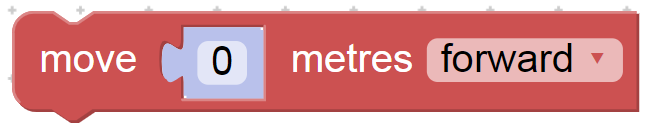
\includegraphics[width=0.3\textwidth]{graphics/blocks/move.png}} & Move \hobbit{} in the given direction \\ \hline
        \raisebox{-\totalheight}{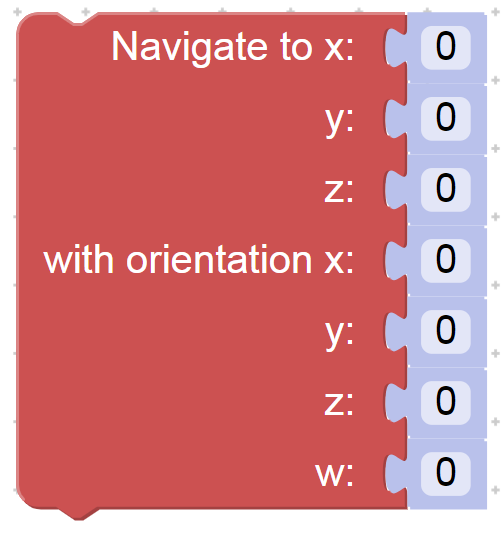
\includegraphics[width=0.3\textwidth]{graphics/blocks/navigation.png}} & Navigate to given pose \\ \hline
        \raisebox{-\totalheight}{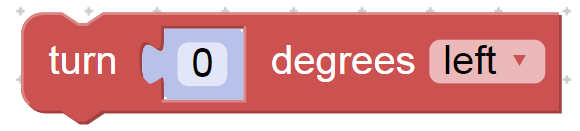
\includegraphics[width=0.3\textwidth]{graphics/blocks/turn.png}} & Rotate \hobbit{} in the given direction \\ \hline
        \raisebox{-\totalheight}{
\includegraphics[width=0.3\textwidth]{graphics/blocks/moveArm.png}} & Move \hobbit{}'s arm to the given position \\ \hline
        \raisebox{-\totalheight}{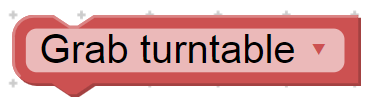
\includegraphics[width=0.3\textwidth]{graphics/blocks/turntable.png}} & Perform the given action with the turntable \\ \hline
        \raisebox{-\totalheight}{
\includegraphics[width=0.3\textwidth]{graphics/blocks/gripper.png}} & Open or close the gripper \\ \hline
        \raisebox{-\totalheight}{
\includegraphics[width=0.3\textwidth]{graphics/blocks/info.png}} & Show an info on \hobbit{}'s tablet \\ \hline
        \raisebox{-\totalheight}{
\includegraphics[width=0.3\textwidth]{graphics/blocks/confirm.png}} & Show an info on \hobbit{}'s tablet and wait for confirmation \\ \hline
        \raisebox{-\totalheight}{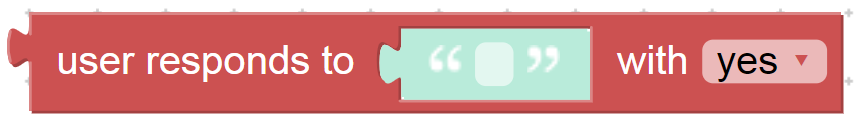
\includegraphics[width=0.3\textwidth]{graphics/blocks/yesno.png}} & Get user's answer to a yes–no question \\ \hline
        \raisebox{-\totalheight}{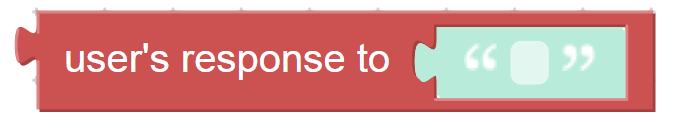
\includegraphics[width=0.3\textwidth]{graphics/blocks/question.png}} & Display the given question on \hobbit{}'s tablet and get user's answer \\ \hline
        \raisebox{-\totalheight}{
\includegraphics[width=0.3\textwidth]{graphics/blocks/headmove.png}} & Move \hobbit{}'s head to the given position \\ \hline
        \raisebox{-\totalheight}{
\includegraphics[width=0.3\textwidth]{graphics/blocks/emotion.png}} & Set \hobbit{}'s eyes according to the given emotion \\ \hline
    \end{tabular}
\end{center}
	% \chapter{ROS reference for \hobbit{}} \label{cha:RefROS}
\begin{table}
	\centering
	\begin{tabular}{l l}
		\toprule
		Message              & Description                    \\
		\midrule
		'center\_center'     & look straight                  \\
		'center\_right'      & look to the right              \\
		'center\_left'       & look to the left               \\
		'up\_center'         & look up                        \\
		'up\_right'          & look to the upper right corner \\
		'up\_left'           & look to the left left corner   \\
		'down\_center'       & look down                      \\
		'down\_right'        & look to the lower right corner \\
		'down\_left'         & look to the lower left corner  \\
		'littledown\_center' & look little down               \\
		'to\_grasp'          & look to grasp position         \\
		'to\_turntable'      & look to turntable              \\
		\bottomrule
	\end{tabular}
	\caption{Possible messages for topic \textit{/head/move}}
	\label{tab:headMoveCommands}
\end{table}
	
	
	% Literaturverzeichnis...
	%=========================
	\printbibliography
	
	
% 	
\chapter*{Erkl�rung}
\thispagestyle{empty}

Hiermit erkl�re ich, dass die vorliegende Arbeit ohne unzul�ssige Hilfe Dritter und ohne Benutzung 
anderer als der angegebenen Hilfsmittel angefertigt wurde. Die aus anderen Quellen oder indirekt 
�bernommenen Daten und Konzepte sind unter Angabe der Quelle gekennzeichnet.
 
Die Arbeit wurde bisher weder im In� noch im Ausland in gleicher oder in �hnlicher Form in anderen 
Pr�fungsverfahren vorgelegt.

\vspace{1.5cm}
 
\noindent\PlaceAndTime

\vspace{1.5cm}
 
 
\noindent\Author
	
	
	% Anzeigen des Seitenlayouts
%	\newpage
%	\layout


\end{document}
